\section{Results}\label{sec:results}

\subsection{Completed experiment and development evidence}
All 128 development and 80 confirmation task runs completed with every
declared candidate present. Independent reconstruction from the saved
forecasts reproduced all 2,496 task--method losses, using targets and
origins identical to the frozen task arrays. The source and diagnostic
freezes remained intact, and all 217 files in the preserved repository
checkpoint were unchanged. The 53 scientific unit tests passed. These
checks establish internal consistency of the supplied implementation and
artifacts; they are not additional evidence about transfer to new sources.

On the development families, raw-plus-KAHM reduced source-balanced scaled
MSE from 3.7827 for raw RBF to 2.1768, a 42.45\% reduction in the aggregated
loss. This average does not describe a broadly shared effect. FRED-MD
accounts for 96.62\% of the net absolute loss reduction. Removing that
family as a descriptive sensitivity analysis reduces the apparent
improvement to 4.65\%. Within FRED-MD, the largest improvement occurs on
series T98. Raw-plus-affine has lower mean error and lower mean wall cost
than raw-plus-KAHM within each of the four development families; its
overall loss is 1.4475. Raw ridge obtains 1.1769. Thus even the favorable
raw-versus-KAHM development comparison does not establish a KAHM-specific
advantage over simpler structural controls.

The development leave-one-family-out diagnostic comparison is likewise
unfavorable to the geometric increment. Metadata plus the validation probe
obtains scaled MSE 2.1720; adding geometry gives 2.1893. Six of 128 choices
change, all from raw to KAHM: two improve their realized loss and four
worsen it. Log-benefit RMSE increases from 1.0121 to 1.0199. These outcomes
were retained, and all four rules were subsequently fitted and frozen
without choosing a preferred rule or changing its decision threshold.
The confirmation phase tests those original rules.

\subsection{Forecast accuracy on reserved sources}
Table~\ref{tab:method-summary} reports every standalone confirmation method.
Raw-plus-KAHM obtains scaled MSE 0.8419, compared with 0.8075 for raw RBF:
the aggregate loss is 4.26\% higher. Raw ridge obtains the lowest
source-balanced mean among the listed standalone candidates, 0.7798.
These are comparisons within the declared small model collection, rather
than a state-of-the-art forecasting claim.

\begin{table}[t]
\centering\small\setlength{\tabcolsep}{4pt}
\caption{Standalone confirmation methods, equally weighted across 4 original source families using the frozen within-source hierarchy. Loss is training-scale-normalized MSE. Wall and CPU seconds cover complete warm-library scientific pipelines. RSS is the averaged maximum recorded process high-water mark, not incremental memory; model size is serialized bytes in KiB. No uncertainty intervals are inferred from dependent tasks.}\label{tab:method-summary}
\begin{tabular}{lrrrrr}
\toprule
Method & Scaled MSE & Wall (s) & CPU (s) & RSS (MiB) & Model (KiB) \\
\midrule
Raw ridge & 0.7798 & 0.188 & 0.1879 & 171.5 & 5.655 \\
Raw RBF & 0.8075 & 0.1688 & 0.1687 & 171.5 & 37.32 \\
Affine local & 0.9449 & 0.5002 & 0.4897 & 171.5 & 93.2 \\
Locality local & 0.8964 & 0.2898 & 0.2898 & 171.5 & 93.4 \\
KAHM local & 0.9354 & 0.3218 & 0.3214 & 171.5 & 164.6 \\
Raw + affine & 0.8458 & 0.3379 & 0.3265 & 171.5 & 107.8 \\
Raw + locality & 0.8462 & 0.2791 & 0.279 & 171.5 & 107.8 \\
Raw + KAHM & 0.8419 & 0.3874 & 0.3814 & 171.5 & 179.2 \\
Seasonal naive & 1.05 & 0.1614 & 0.1613 & 171.5 & 0.1382 \\
Holt & 2.373 & 0.3449 & 0.3446 & 171.5 & 0.4219 \\
Histogram boosting & 0.9555 & 8.91 & 8.901 & 171.5 & 2591 \\
MLP & 0.8785 & 1.463 & 1.462 & 171.5 & 71.62 \\
\bottomrule
\end{tabular}
\end{table}


Figure~\ref{fig:source-gains} shows why the comparison must be read at the
source level. Relative to raw RBF, raw-plus-KAHM increases mean loss by
0.50\% on Traffic, 12.27\% on Hospital, and 3.53\% on US Births. It reduces
mean loss by 1.53\% on Saugeen river flow, from 0.6106 to 0.6012; raw ridge
obtains 0.5220 on that same source. Removing any one confirmation family
still leaves raw-plus-KAHM with a higher aggregate loss than raw RBF.
The source-level conclusion is therefore not caused solely by the largest
Hospital degradation, although the size of the effect depends on the
family mixture.

\begin{figure}[t]
\centering
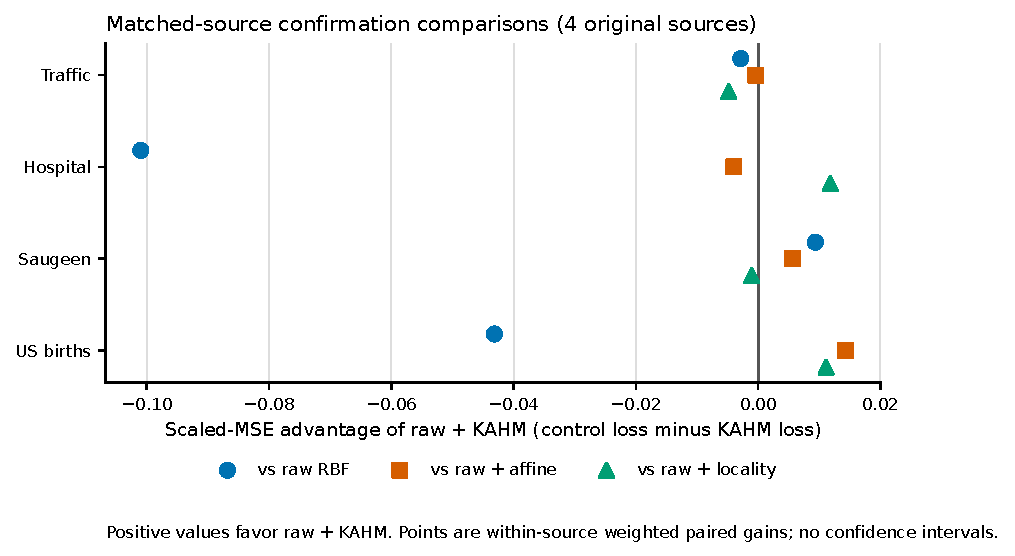
\includegraphics[width=\linewidth]{generated/figures/source_gains.pdf}
\caption{Within-source confirmation comparisons. Positive differences favor
raw-plus-KAHM. The plotted points are paired differences of the same
hierarchically weighted source means, not independent-window estimates.
The KAHM advantage over structural controls is small and changes sign
across sources.}\label{fig:source-gains}
\end{figure}

The raw-plus-affine and raw-plus-locality controls obtain 0.8458 and
0.8462, respectively. Raw-plus-KAHM improves on these aggregate values
by only 0.46\% and 0.50\%, with each comparison favoring KAHM in two
family means and the control in two. These small, mixed aggregate differences
do not establish that nonlinear reconstruction is the relevant mechanism.
The controls without
raw augmentation obtain losses 0.9449 for affine, 0.8964 for locality,
and 0.9354 for KAHM. Retaining the complete raw history helps the
aggregate performance of each local code here, but does not make the
augmented KAHM procedure superior to the raw-history baseline.

Capacity changes the magnitude of the result. At the small setting,
raw-plus-KAHM obtains 0.8551 versus raw RBF's 0.8383, about 2.00\% worse.
At the medium setting it obtains 0.8288 versus 0.7767, about 6.70\% worse.
Its small aggregate advantage over raw-plus-affine reverses at the medium
setting. The cap on training windows and the model sizes change together,
and the former binds only for the long confirmation series; this experiment
does not isolate their individual effects.

\subsection{Accuracy and complete measured computational cost}
Raw-plus-KAHM costs 0.3874 seconds per hierarchically weighted confirmation
task, compared with 0.1688 seconds for raw RBF, a factor of 2.30.
Raw ridge obtains lower mean loss than either at 0.1880 seconds. KAHM's
small aggregate improvements over raw-plus-affine and raw-plus-locality
come with 14.65\% and 38.82\% greater mean wall cost, respectively.
Figure~\ref{fig:accuracy-cost} plots these observed tradeoffs together
with the decision procedures. The measurements do not imply fixed
hardware-independent speed ratios, and individual source/capacity timings
can differ from the aggregate order.

Implementation overhead is material for these small fits. In particular,
selection cleanup, including explicit garbage collection, accounts for
0.1381 of raw RBF's 0.1688 seconds and 0.1825 of raw-plus-KAHM's
0.3874 seconds. Their search computations take 0.0130 and 0.1113 seconds,
and their final refits take 0.0051 and 0.0724 seconds, respectively.
The complete measured totals include this cleanup consistently. The
reported 2.30-fold ratio describes the supplied fitting workflow,
not an intrinsic arithmetic complexity ratio between feature maps.
Table~\ref{tab:cleanup-costs} separates cleanup and the launch-to-result
measurements for the matched pair.
\begin{table}[t]
\centering\small\setlength{\tabcolsep}{4pt}
\caption{Confirmation cost transparency for the primary matched pair, with equal source-family weighting. Total is the complete warm-library scientific pipeline. Cleanup is its measured selection-overhead component, including explicit garbage collection; the percentage is the ratio of aggregated component and total times. Launch separately reports the measured isolated-child launch-to-result interval. These are implementation-specific costs, not intrinsic kernel arithmetic or universal complexity ratios.}\label{tab:cleanup-costs}
\begin{tabular}{lrrrr}
\toprule
Method & Total (s) & Cleanup (s) & Cleanup (\%) & Launch (s) \\
\midrule
Raw RBF & 0.16879 & 0.13808 & 81.8 & 0.17748 \\
Raw + KAHM & 0.38741 & 0.18253 & 47.11 & 0.40097 \\
\bottomrule
\end{tabular}
\end{table}


\begin{figure}[t]
\centering
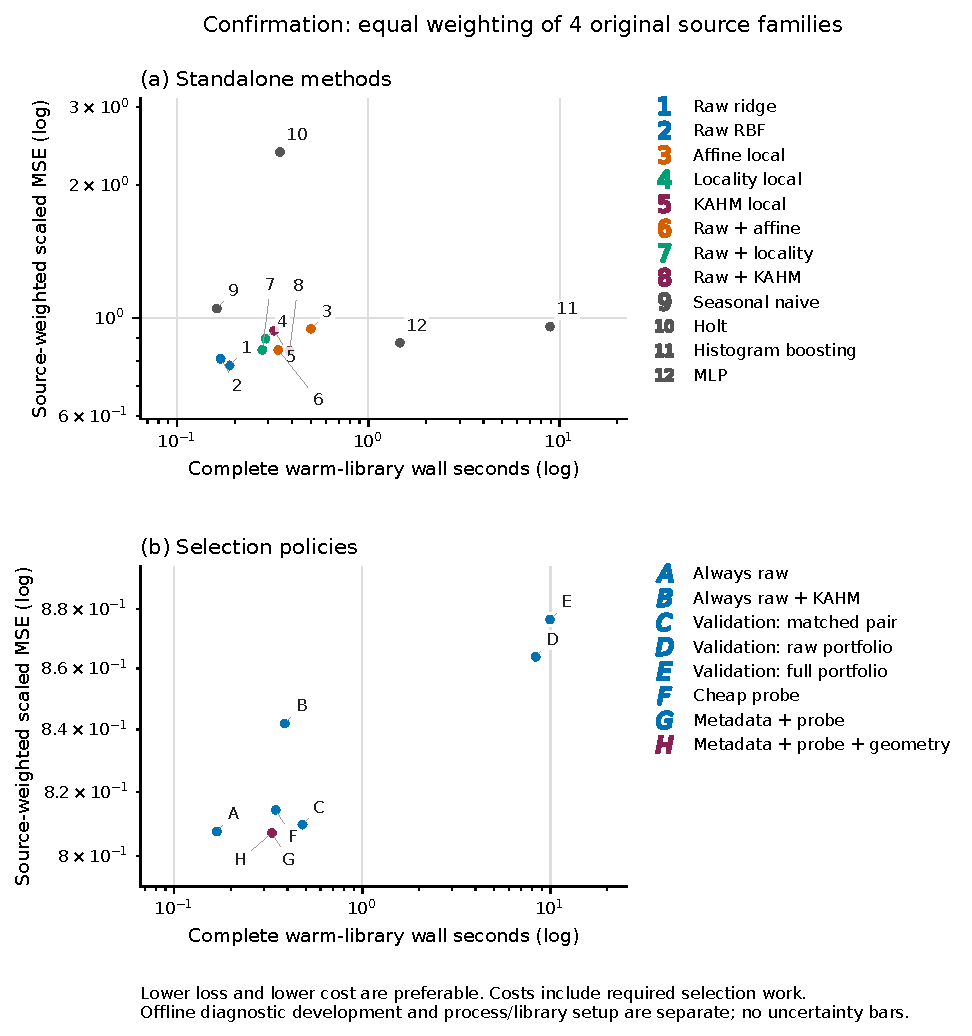
\includegraphics[width=\linewidth]{generated/figures/accuracy_cost.pdf}
\caption{Confirmation accuracy and warm-library scientific-pipeline cost.
All points use the same source hierarchy. The standalone and selector
panels have independently chosen scales to keep the full declared
comparisons visible. Selector costs include the searches and probes
needed to choose a model. No method is selected using the confirmation
outcomes for deployment.}\label{fig:accuracy-cost}
\end{figure}

The cost records include preprocessing, validation search with
within-method alpha-path reuse, final refitting, forecasting, and model
serialization. They separately expose the child launch-to-result interval
and library initialization. The two freeze processes recorded shared
library import costs of 8.724 and 4.873 seconds; these are distinct
measurements, not per-task charges or a claim that one method requires
every imported library. Across both phases, the sum of recorded task
intervals is 1,565.56 seconds (26.09 minutes), including every benchmarked
candidate, probe, orchestration, and prediction export. It excludes
unmeasured preparation intervals and pauses between stages.

Process high-water RSS averages 171.5 MiB for every standalone confirmation
method in this run. That common interpreter/input-dominated high-water
mark does not resolve incremental memory differences. Serialized model
sizes do differ: raw RBF averages 37.32 KiB, raw-plus-KAHM 179.2 KiB,
and raw ridge 5.655 KiB. A saved model's byte count should not be confused
with the memory needed to fit or query it.

The MLP baseline is also bounded by its declared iteration cap: 68 of
80 selected confirmation refits reach it. All such fits and warnings are
retained. No candidate exceeded the execution limits or was omitted.
The manuscript therefore compares the specified finite procedures;
it does not claim an optimally trained MLP or an optimized implementation
of every alternative.

\subsection{Does the frozen diagnostic identify useful KAHM cases?}
The primary increment, metadata-plus-probe-plus-geometry versus
metadata-plus-probe, changes none of the 80 confirmation decisions.
Both rules obtain scaled MSE 0.807085 and select raw-plus-KAHM on
31.25\% of the source-weighted task mass. Their mean warm-library costs
are both about 0.3309 seconds. The few microseconds separating their
recorded decision times have no practical interpretation. The geometric
features are already obtained from the paid KAHM probe, so this comparison
does not require an additional representation fit.

\begin{table}[t]
\centering\small\setlength{\tabcolsep}{4pt}
\caption{Frozen-policy confirmation outcomes over 4 source families with the same hierarchical weighting. Gain is raw-RBF scaled MSE minus chosen loss. Harm is the weighted fraction with loss more than 5\% above raw RBF. The final column counts selection of the specific raw-plus-KAHM pair member, including in portfolios. Wall cost includes all required probes/searches and decision inference, then the chosen final refit, forecast and model serialization. Offline evidence acquisition and diagnostic fitting are separate.}\label{tab:policy-summary}
\begin{tabular}{lrrrrr}
\toprule
Policy & Scaled MSE & Wall (s) & Gain & Harm (\%) & Raw+K (\%) \\
\midrule
Always raw & 0.8075 & 0.1688 & 0 & 0 & 0 \\
Always raw + KAHM & 0.8419 & 0.3874 & -0.0344 & 25 & 100 \\
Validation: matched pair & 0.8097 & 0.4812 & -0.002159 & 5.47 & 32 \\
Validation: raw portfolio & 0.8639 & 8.338 & -0.05638 & 10.9 & 0 \\
Validation: KAHM family & 0.8406 & 0.6242 & -0.03306 & 26.6 & 73.4 \\
Validation: full portfolio & 0.8764 & 9.948 & -0.0689 & 14.8 & 14.1 \\
Cheap probe & 0.8143 & 0.3465 & -0.006771 & 9.38 & 50 \\
Metadata & 0.816 & 0.2976 & -0.008445 & 15.6 & 50 \\
Metadata + geometry & 0.816 & 0.3695 & -0.008445 & 15.6 & 50 \\
Metadata + probe & 0.8071 & 0.3309 & 0.0004363 & 3.12 & 31.2 \\
Metadata + probe + geometry & 0.8071 & 0.3309 & 0.0004363 & 3.12 & 31.2 \\
\bottomrule
\end{tabular}
\end{table}


The identical decisions do not imply identical benefit estimates.
Log-benefit RMSE increases slightly, from 0.184549 without geometry to
0.184680 with it, and weighted sign accuracy is 58.59\% for both.
Always predicting that KAHM will not improve on raw has sign accuracy
61.72\% on these weighted confirmation tasks. This constant comparison
is descriptive and was not used to alter the frozen rule. Metadata-plus-
geometry also makes exactly the same choices as metadata alone, while
paying for its extra feature acquisition. Estimated-benefit errors and
fixed coefficients are reported in Appendix~\ref{app:full-results}.

\begin{figure}[t]
\centering
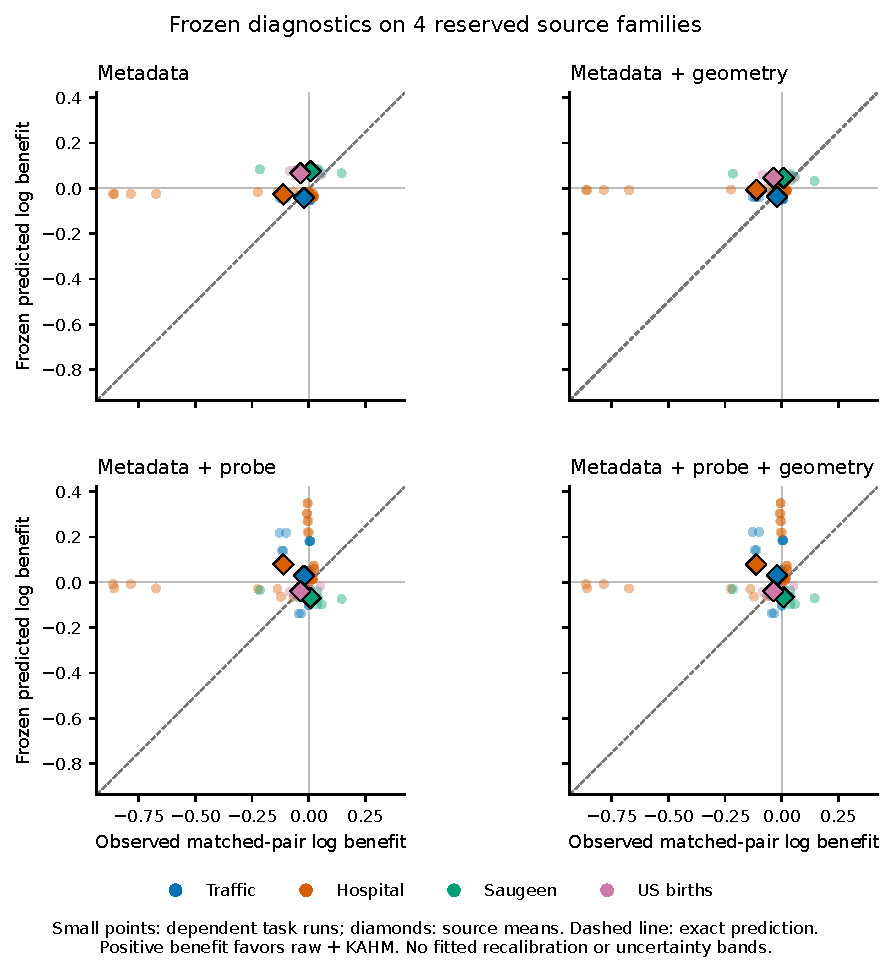
\includegraphics[width=0.92\linewidth]{generated/figures/diagnostic_predictions.pdf}
\caption{Observed versus frozen predicted log benefit for all four
diagnostics. Points within a source are dependent task runs; diamonds
show source means. Estimates are neither recalibrated on confirmation
data nor interpreted as probabilities. Similar selection decisions can
coexist with different estimated magnitudes.}\label{fig:diagnostic-predictions}
\end{figure}

The probe-based diagnostic's aggregate reduction from always-raw loss is
0.000436, or 0.054\%, at 1.96 times the raw predictor's pipeline cost.
It improves one source mean, worsens one, and ties two. It is better than
always choosing KAHM and better on these aggregates than the cheap-probe
decision or full validation portfolios. Those comparisons do not establish
the geometric increment or a practically useful gain over always raw.
The raw and full validation portfolios cost 8.338 and 9.948 seconds,
respectively, while obtaining losses 0.8639 and 0.8764. Counting every
candidate search prevents their choice of a comparatively inexpensive
final forecaster from concealing the cost of selection.

Offline learning is a separate investment. Acquiring the development
labels from the matched raw/KAHM pair costs a sum of 68.41 seconds of
standalone scientific-pipeline work. Adding the shared metadata/probe
dependencies gives 80.83 seconds; the four final diagnostic ridge fits
together add 0.032 seconds. These dependencies can be shared across
variants, so their separate acquisition totals must not be added.
The bookkeeping conservatively repeats preparation where cross-task
caching could be possible. Reporting only the millisecond-scale ridge
fits would substantially understate the measured cost of obtaining the
diagnostic. No invented number of future deployments is used to
amortize that investment.
